%!TEX root = ../marisa-thesis.tex
\chapter{Combinatorics and Its Applications}
The foundation of the research stems from the Combinatorial Trace Method and the Graph Theory used to further claims and understand concepts.\\

The \textbf{combinatorial trace method} is complex and therefore certain mathematical properties, operations, etc. need to be understood and defined before any further study.
\cite{CombinatorialArticle}
Using these concepts we can take certain properties of graphs and apply it to the graphs explored throughout the research.  Through these properties and observations we can review back and compare the graphs that are being explored and the general rules and properties it already has from the shape, the vertices, etc. 

\section{Applying the Definitions}
Throughout the research, closed walks are explored for different graphs.  Let us look at the closed walks in figure 2.1.

For example, the following matrix, $A$, is an adjacency matrix for the graph:\\
\begin{figure}[h]
         \centering
         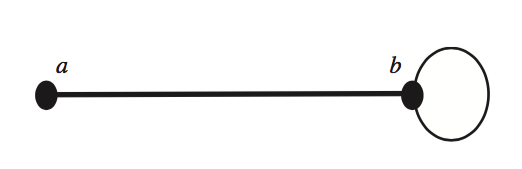
\includegraphics[width = 2.0in]{CMT2.png}
         \caption{\small{A graph of two vertices}}
 \end{figure}

  $$
\begin{bmatrix} 
     0        &         1     \\
     1        &         1      \\

\end{bmatrix}
$$
This demonstrates a matrix that corresponds to the total number of walks of length one. This does not show the amount of closed walks. 

The trace for the matrix $A$ shown above would be equal to 1. The diagonal of the trace is from the top left to the bottom right entry. Here there are only two entries.  Thus, the calculation would be:

\begin{align*}
    0+1=1
\end{align*}
Therefore, the trace is equal to 1. Thus, there is one closed walk of length $n$ for this graph.

Moreover, the eigenvalue and eigenvectors can be found from this matrix. The determinant equation will be used to find the eigenvalues. 

\begin{proposition}
    The determinant of the eigenvalues of the adjacency matrix give the total number of closed walks within the graph of a given length.
\end{proposition}

We can analyze this proposition:\\
\begin{equation}
det(A-\lambda~I) = 0 
\end{equation} 


\[
\begin{bmatrix} 
     0        &         1     \\
     1        &         1      \\

\end{bmatrix}
-
\begin{bmatrix}
\lambda &        0 \\
0          &        \lambda\\    

\end{bmatrix}
\]


The eigenvalues evaluated to be 
\begin{align*}
    \lambda_1 = \frac{1+\sqrt{5}}{2}, \lambda_2 = \frac{1-\sqrt{5}}{2}
\end{align*}

\par The eigenvalues and eigenvectors showcase the total number of closed walks. We can use these eigenvalues and put them to the power of $n$, length, and add them to find the total number of closed walks. 
\\For example, 
the total number of walks within a graph of the given length is represented below:
\begin{align*}
= \lambda_1^3+\lambda_2^3 \\
= (\frac{1+\sqrt{5}}{2})^3 + (\frac{1-\sqrt{5}}{2})^3 = 4
\end{align*}
Thus, there are 4 total number of walks within the given length of 3 in this graph. We will explore this further in the next chapter.

\begin{theorem}
    Graphs without loops do not have a closed walk of length 1.
\end{theorem}
Let us look at figure 2.3. 
\begin{figure}[h]
         \centering
         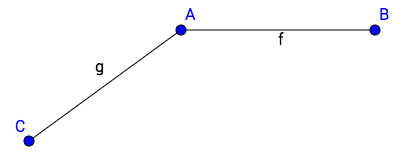
\includegraphics[width = 2.0in]{degree.png}
         \caption{\small{\color{red}Figure 2.3 repeated}}
 \end{figure}
We can look at the figure and contemplate different walks we can take. For example, the walk from vertex C to vertex A exists, but the walk from vertex B to vertex C does not exist because there is no edge to connect them. Can we make any closed walks? \\
Yes, we can walk a walk of length 2 from vertex A to vertex B back to vertex A. Vertex A cannot return to itself with a length of one walk.  
\par Let us assume there exists a closed walk of length 1. Since the only edges that exist within the graph are connected to the center vertex, A, that edge is counted twice.  Therefore, the edge cannot be used.  Thus, there are no walks without a loop, which connects a vertex to itself.
\begin{proposition}
    Graphs without a cycle do not have any total number of odd closed walks.
\end{proposition}
The condition onto the graph, $G$, is that there are only a total number of closed walks of even length. The condition must be followed by all the subsets of $G$, and $G$ itself.

\begin{proof}
    For graphs with less than a cardinality of $G$ edges $(|E(G)|)$ the statement holds.
    Let us look at $H$ as a subset of $G$.  Therefore, the condition carries to $H$, that there cannot exist a total number of odd closed walks.  Let there be closed even walks on $v_{j}$ by the inductive hypothesis. 
    \par
    Let $v_{i}$ take an edge to $v_{j}$, then $v_{j}$ takes an edge that is not connected to $v_{i}$, thus $v_{j}$ must make a closed walk that is even because there is no cycle within. \\
    \par 
    \textbf{Base Case:} Let us have a graph with 2 vertices, keep adding edges to the graph.  Thus, the base case is satisfied because although adding edges, it is still a subset of $G$, which means the subset inherits the condition that there are no total number of odd closed walks. \\
    \begin{center}
        \textbf{IH:} For graphs with less than $(|E(G)|)$ edges, keep adding edges and assume it works for the small graph. 
    \end{center}
    
    \par
    Then $G$ can take any path and any vertex, but still has to encounter them twice because of the condition. Thus, let us remove an edge ad have it have 1 less edge.  By the condition, $v_{j}$ must have an even number of total closed walks, because although only removed one edge, two walks along that edge were eliminated.  Moreover, if the edge that was removed is added back, the edge will bring bacck a plus 2 number of walks.  Therefore, it will force the condition back onto $G$.
\end{proof}

From this proof, we know that any subsets of the same symmetric graph hold the same condition, therefore, it is expected that the rest of the hydrocarbons do not have an odd total number of closed walks. 

\section{The Combinatorial Trace Method in Action}
At the beginning of the research, the paper ``The Combinatorial Trace Method in Action'' was utilized and evaluated for further understanding of the world of combinatorics and how there can be different uses for the method. 

\par If we look at the figure that was presented from the paper: \textit{``The Combinatorial Trace Method in Action"}

Krebs and Martinez demonstrate the figure shown below. 

\begin{figure}[h]
         \centering
         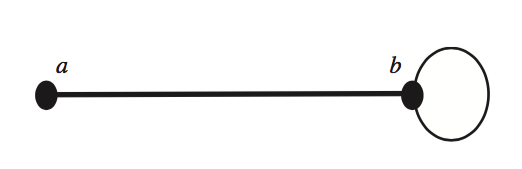
\includegraphics[width = 2.0in]{CMT2.png}
         \caption{\small{The Combinatorial Trace Method in Action Example}}
 \end{figure}

The Combinatorial Trace Method in Action continues the idea stated previously with eigenvalues, eigenvectors, adjacency matrices, etc. with the Fibonacci sequence and Lucas numbers.

\par The team used the Binet Formula 
\begin{align*}
    L_n = \phi^n + \phi^{-n}
\end{align*}
This equation yielded \\
\begin{align*} 
    \phi = \frac{1+\sqrt{5}}{2}, \bar\phi= \frac{1-\sqrt{5}}{2}
\end{align*}
The form of this equation-a combinatorial expression on the left and a power sum on the right-immediately suggests that the combinatorial trace method is applicable for an appropriate graph. This graph consists of two vertices $a$ and $b$ with an edge between them and a loop at $b$. 

%\begin{figure}[h]
 %        \centering
 %        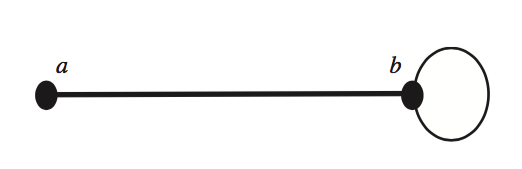
\includegraphics[width = 2.0in]{CMT2.png}
 %        \caption{\small{The Combinatorial Trace Method in Action}}
 %\end{figure}

 The walks that are $\geq 2$ walks at $b$ can either be back and forth along the edge or going around the loop. Hence the formula 
 \begin{align*}
     B_n = B_{n-1} + B_{n-2}     
 \end{align*}
 By definition of the Fibonacci numbers, it can be said that $B_n = F_{n+1}$
 Continuing this pattern, the number of closed walks of length 0 beginning at $a$ is equal to 1 which is equal to $F_{-1}$.  Moreover, the number of closed walks of length 1 is equal to 0, thus is equal to $F_0$.  For all the closed walks $\geq 2$, consists of back and forth along the edge and around the loop at $b$ with a closed walk of length $n-2$.  Therefore, it gives the closed walks of length $n$ to be equal to $B_{n-2} = F_{n-1}$. 
 \par The identity of the Lucas numbers is: $L_n = F_{n+1} + F_{n-1}$ it was found that the total number of closed walks in the graph of length n was $L_n = A_{n} + B_{n}$. This would include that the adjacency matrix would be the one given above and restated below. 

  $$
\begin{bmatrix} 
     0        &         1     \\
     1        &         1      \\

\end{bmatrix}
$$
 with the eigenvalues stated previously. Therefore, this ensures a concrete path to finding a graph from an adjaceny matrix and its eigenvalues or vice versa, where the graph can help find the adjaceny matrix and the eigenvalues.

Let us think about our previous proposition:

\begin{proposition}
    The determinant of the eigenvalues of the adjacency matrix give the total number of walks within the graph of a given length. 
\end{proposition}

To further demonstrate this idea we can look at another example. 
\par Let us evaluate the graph given previously.\\\\\\\
\begin{figure}[h]
         \centering
         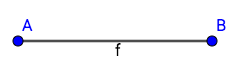
\includegraphics[width = 2.0in]{vertices.png}
         \caption{\small{Another graph}}
 \end{figure}

We can create an adjacency matrix for the graph based on the number of vertices we have.  Thus, the matrix will be a $2\times2$ matrix. 

$$
\begin{bmatrix}
     w        &         x     \\
     y        &         z      \\
\end{bmatrix}
$$
We will look for the total number of closed walks of length 1. 
\par
Looking at the first spot of the matrix, $a_{1,1}$, (denoted $w$), we evaluate whether there is a closed walk of length one from vertex $A$ to itself. There does not exist such a walk therefore we will put a 0 in that spot.


$$
\begin{bmatrix}
     0        &         x     \\
     y        &         z      \\
\end{bmatrix}
$$

Moreover, the next spot $x$ is a closed walk of length 1 from vertex $A$ to vertex $B$. There is a walk that exists, thus, the number would be 1. 

$$
\begin{bmatrix}
     0        &         1     \\
     y        &         z      \\
\end{bmatrix}
$$

In addition, we can continue in this fashion and find:

$$
\begin{bmatrix}
     0        &         1     \\
     1        &         0      \\
\end{bmatrix}
$$
Thus, this would be the resulting matrix.

\[
\begin{bmatrix}
     0        &         1     \\
     1        &         0      \\
\end{bmatrix}
- 
\begin{bmatrix}
     \lambda        & 0     \\
     0        &         \lambda      \\
\end{bmatrix}
\]


$$
\det\begin{bmatrix}
-\lambda & 1 \\
1 & -\lambda \\
\end{bmatrix}
$$
This would yield $\lambda^2 -1$ which equals \\
\begin{align*}
    (\lambda + 1)(\lambda - 1) =0 \\
    \lambda = \pm 1 
\end{align*}
Thus, the eigenvalues were evaluated using the adjacency matrix and its determinant. 
